% Microeconomics problem set (English, university), with a pgfplots supply-and-demand graph.
% Headings: "Problem N --- Title --- P points" in bold (em dashes, points as the last words); parts (a), (b), ...
\documentclass[11pt,a4paper]{article}
\usepackage[T1]{fontenc}
\usepackage{lmodern}
\usepackage[margin=2.3cm,top=2.0cm,bottom=2.2cm]{geometry}
\usepackage{amsmath,amssymb}
\usepackage{caption}
\usepackage{tikz}
\usepackage{pgfplots}
\pgfplotsset{compat=1.18}
\usepackage{enumitem}

\setlength{\parindent}{0pt}
\setlist[enumerate,1]{label=(\alph*), leftmargin=2.2em, itemsep=0.35em, topsep=0.3em}
\newcommand{\problem}[3]{\bigskip\par\noindent\textbf{Problem #1 --- #2 --- #3 points}\par\nopagebreak\smallskip}

\begin{document}

% ---- header ---------------------------------------------------------------------------
{\small ECON 1010 \textperiodcentered{} Principles of Microeconomics \hfill Department of Economics}\\[-0.4em]
\rule{\linewidth}{0.6pt}\\[0.5em]
{\Large\bfseries Problem Set 3: Markets, Elasticity and Taxes}\\[0.4em]
Due: Thursday, November 19, 2026 \hfill Total: 34 points\\[0.3em]
{\small Prices are in dollars per unit, quantities in units per week. Show your work.}

% ---- Problem 1 ------------------------------------------------------------------------
\problem{1}{Market equilibrium}{10}
In the market for a good the demand and supply curves are $Q_d = 100 - 2P$ and $Q_s = -20 + 4P$.
Figure~1 plots the inverse curves: demand $P = 50 - Q/2$ and supply $P = 5 + Q/4$.

\begin{center}
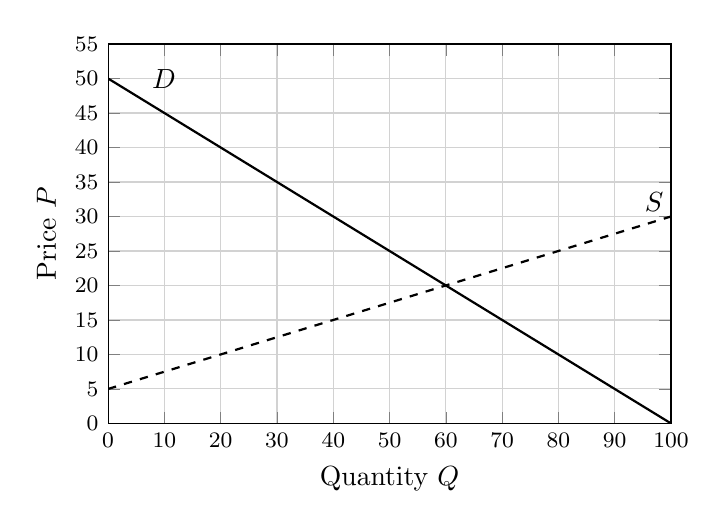
\begin{tikzpicture}
\begin{axis}[width=0.72\linewidth, height=6.4cm,
    xlabel={Quantity $Q$}, ylabel={Price $P$},
    xmin=0, xmax=100, ymin=0, ymax=55,
    xtick distance=10, ytick distance=5, grid=both,
    major grid style={gray!35}, minor grid style={gray!10},
    tick label style={font=\footnotesize}]
  \addplot[thick, domain=0:100] {50 - x/2} node[pos=0.06, above right] {$D$};
  \addplot[thick, dashed, domain=0:100] {5 + x/4} node[pos=0.97, above] {$S$};
\end{axis}
\end{tikzpicture}
\captionof{figure}{Demand ($D$) and supply ($S$) in the market.}
\end{center}
\begin{enumerate}
  \item Read the equilibrium price and the equilibrium quantity from Figure~1. (2 points)
  \item Check your reading by solving $Q_d = Q_s$ algebraically. (3 points)
  \item The government imposes a price ceiling of \$15. Find the quantity demanded, the quantity supplied
        and the size of the shortage. (3 points)
  \item Explain in one sentence why the price ceiling is binding. (2 points)
\end{enumerate}

% ---- Problem 2 ------------------------------------------------------------------------
\problem{2}{Price elasticity of demand}{8}
Use the demand curve $Q_d = 100 - 2P$ from Problem~1.
\begin{enumerate}
  \item Compute the point price elasticity of demand at the equilibrium of Problem~1. (3 points)
  \item Compute the midpoint (arc) elasticity when the price rises from \$20 to \$25. (3 points)
  \item Is demand elastic or inelastic in this range? What happens to total revenue when the price rises
        from \$20 to \$25? (2 points)
\end{enumerate}

% ---- Problem 3 ------------------------------------------------------------------------
\problem{3}{A per-unit tax}{10}
The government now levies a tax of $t = \$6$ per unit, paid by the sellers. Demand and the original
supply curve are as in Problem~1.
\begin{enumerate}
  \item Find the new supply curve (in terms of the price $P_c$ paid by consumers), the new equilibrium
        quantity, the price paid by consumers and the price received by sellers. (4 points)
  \item How much of the tax per unit is borne by consumers and how much by producers? (2 points)
  \item Compute the tax revenue of the government. (2 points)
  \item Compute the deadweight loss of the tax. (2 points)
\end{enumerate}

% ---- Problem 4 ------------------------------------------------------------------------
\problem{4}{Consumer surplus}{6}
Return to the inverse demand curve $P = 50 - Q/2$.
\begin{enumerate}
  \item Compute the consumer surplus in the market equilibrium without the tax. (2 points)
  \item Compute the consumer surplus after the tax of Problem~3 has been introduced. (2 points)
  \item By how much does the consumer surplus fall? (2 points)
\end{enumerate}

\end{document}
